\section{Topological Spaces}

`Do continuity entirely in terms of open sets without mentioning distance'.

Metric space: set with a distance.

Topological space: set with a collection of open subsets.

\subsection{Definitions and Examples}

\begin{definition}[Topological Space]
    A \vocab{topological space} is a set $X$ endowed with a \vocab{topology} $\tau$ that is a subset $\tau \subset \mathcal{P}(X)$ satisfying
    \begin{enumerate}
        \item $\emptyset \in \tau$ and $X \in \tau$;
        \item If $\sigma \subset \tau$ then $\bigcup_{G \in \sigma} G \in \tau$;
        \item If $G_1, \dots, G_n \in \tau$ then $\bigcap_{i = 1}^n G_i \in \tau$.
    \end{enumerate}
\end{definition}

\begin{remark}
    Could replace (3) by $G, H \in \tau \implies G \cap H \in \tau$.
    Equivalent to (3) by induction.
\end{remark}

\begin{notation}
    Sometimes write `$(X, \tau)$ is a topological space'.
    If obvious what the topology is, we might just write `$X$ is a topological space'.
\end{notation}

\begin{example}
    Let $(X, d)$ be a metric space.
    Let $\tau = \{G \subset X : G \text{ open}\}$.
    Then by \cref{prp:26}, $\tau$ is a topology on $X$.

    We say $\tau$ is the \underline{topology, induced by the metric $d$}.
\end{example}

We want to define open/ closed/ cts etc for topological spaces.
As metric spaces are top. spaces try to make sure it's `backward compatible', so to say.
The new defns shouldn't contradict the old metric space ones.
So in making new defns, we'll be guided by section 2.4.

\begin{definition}[Open]
    Let $(X,\tau)$ be a topological space. We say that $G\subset X$ is \vocab{open} if $G\in \tau$
\end{definition}

\begin{definition}[Closed]
    Let $(X,\tau)$ be a topological space.
    We say $F$ is \vocab{closed} if $X  \setminus F \in\tau$.
\end{definition}

\begin{definition}[Neighbourhood]
    Let $(X,\tau)$ be a topological space.
    We say $\mathcal{N} \subset X$ is a \vocab{neighbourhood} of $a\in X$ if $\exists G\subset X$ open with $a\in G\subset \mathcal{N}$.
\end{definition}

\begin{definition}[Continuity]
    Let $(X,\tau)$ be a topological space.
    Let $(Y,\sigma)$ be another topological space, and let $f:X \to Y$. We say $f$ is \vocab{continuous} if whenever $G\subset Y$ is open, then $f\inv(G)\subset X$ is open.
    In other words, $f$ is continuous if $\forall \; G \in \sigma, f\inv(G) \subset \tau$.

    We say that $f$ is \vocab{continuous at $a \in X$} if whenever $\mathcal{N} \subset Y$ is a neighbourhood of $f(a)$ then $f\inv(\mathcal{N})\subset X$ is a neighbourhood of $a$.
\end{definition}

\begin{definition}[Homeomorphisms]
    Let $(X,\tau)$ be a topological space.
    We say that $f$ is a \vocab{homeomorphism} and $X,Y$ are \vocab{homeomorphic} if $f$ is a bijection and both $f,f\inv$ are continuous.
\end{definition}

\begin{definition}[Topological]
    Let $(X,\tau)$ be a topological space.
    A property is \vocab{topological} if it is preserved by homeomorphisms; that is to say, if $X,Y$ are homeomorphic then $X$ has the property iff $Y$ does.
\end{definition}

\begin{remark}
1. if $\tau$ is induced by a metric then this is all consistent with the metric space definitions of these concepts.

2. Given our definition, $G$ open iff $G\in \tau$, we often don't need to explicitly name the topology.
E.g. `Let $X=\R$ with the usual topology and $G\subset X$ be open\dots'.
Other times more convenient to specify $\tau$, write `$G\in \tau$' etc.

3. Homeomorphism is an equivalence `relation'.

4. If $a\in G$ and $G$ open then $G$ is a neighbourhood of $a$, however neighbourhoods need not be open in general. A set $G\subset X$ is open iff $G$ is a neighbourhood of each of its points.
\end{remark}

\begin{proposition} \label{prp:27}
Let $X,Y$ be topological spaces and $f: X \to Y$. Then $f$ is continuous if and only if for all $a\in X$, $f$ is continuous at $a$.
\end{proposition}

\begin{proof}
($\implies$): Suppose $f$ continuous and let $a\in X$. Let $\mathcal{N}\subset Y$ be a neighbourhood of $f(a)$.
Then there is an open set $G\subset Y$ with $a\in G\subset \mathcal{N}$.
As $f$ is continuous, $f\inv(G)\subset X$ is open.
Now $a\in f\inv(G) \subset f\inv(\mathcal{N})$ with $f\inv(G)$ open. Thus $f$ is continuous at $a$.

($\Longleftarrow$): Suppose for all $a \in X$ we have $f$ continuous at $a$.
Let $G\subset Y$ be open.
Let $a \in f\inv(G)$.
Then $f(a) \in G$, but $G$ is open so $G$ is a neighbourhood of $f(a)$.
Now $f$ is continuous at $a$ so $f\inv(G)$ is a neighbourhood of $a$ in $X$.
But $a$ was arbitrary so $f\inv(G)$ is a neighbourhood of each of its points.
That is $f\inv(G)$ is open.
Hence $f$ is continuous.
\end{proof}

\begin{proposition} \label{prp:28}
Let $(X,\tau), (Y,\sigma), (Z,\rho)$ be topological spaces, let $f:X \to Y$ and $g:Y \to Z$ be continuous. Then $g\circ f: X \to Z$ is continuous.
\end{proposition}

\begin{proof}
Let $G\in \rho$. As $g$ is continuous, $g\inv(G)\in \sigma$. As $f$ continuous, $f\inv(g\inv(G))\in \tau$. That is, $(g\circ f)\inv(G)\in \tau$. So $g\circ f$ continuous.
\end{proof}

\begin{example}[The discrete topology]
    Let $X$ be any set and $\tau = \mathcal{P}(X)$, where `every set is open'. \\
    However, this is not a new example; it is induced by the discrete metric \begin{align*}
        d(x, y) = \begin{cases}
            1 & x \neq y \\
            0 & x = y
        \end{cases}.
    \end{align*}
    Now in $(X,d)$, for any $x\in X$ then $\{x\} = B_1(x)$ is open and so if $G\subset X$ then $G = \bigcup_{x\in G} \{x\}$ is open.
\end{example}

\begin{example}[The indiscrete topology]
    Let $X$ be any set and $\tau = \{\emptyset, X\}$. Here, `only open sets are $\emptyset$ and whole space'.
    This is something we have not seen before: $\tau$ cannot be induced by a metric as long as $|X| \geq 2$.
    Indeed, suppose $|X|  \geq 2$ and that $\tau$ is induced by a metric $d$.
    Let $x,y \in X$ with $x\neq y$, so let $d(x,y) = \delta>0$.
    Then $B_\delta(x)$ is open with $x \in B_\delta(x)$ and $y \not\in B_\delta(x)$ \Lightning.
\end{example}

\begin{example}[The cofinite topology]
    Let $X$ be any infinite set and let $\tau = \{G\subset X : X \setminus G \textup{ is finite} \} \cup \{\emptyset\}$.
    This is not induced by a metric.

    \begin{proof}
        \begin{enumerate}
            \item $\emptyset\in\tau$ and $X \setminus X = \emptyset$ is finite so $X\in\tau$.
            \item Let $\sigma \subset\tau$. If $\sigma$ is empty or only contains $\emptyset$ then $\bigcup_{G\in \sigma} G = \emptyset\in \tau$.
            Otherwise, pick $H\in \sigma$ with $H\neq \emptyset$. Then $X \setminus H$ is finite so $(X \setminus\bigcup_{G\in \sigma} G) = \bigcap_{G\in \sigma} (X \setminus G)\subset X \setminus H$ is finite. So $\bigcup_{G\in \sigma} G \in \tau.$
            \item Let $G,H\in \tau$. If $G = \emptyset$ or $H=\emptyset$ then $G\cap H = \emptyset\in\tau$. Otherwise $X \setminus G, X \setminus H$ are finite then $(X \setminus(G\cap H)) = (X \setminus G)\cup(X \setminus H)$ is finite. So $G\cap H\in \tau$.
        \end{enumerate}

        So the cofinite topology is indeed a topology.

        Furthermore, it is not induced by a metric $d$.
        Observe first that if $G,H$ open and non-empty then $G\cap H\neq \emptyset$\footnote{As they are both infinite sets with finite complements}.
        Now suppose $x, y \in X$ with $x \neq y$.
        Then $d(x,y) = \delta > 0$ so $B_\delta/2(x), B_\delta/2(y)$ are non-empty disjoint open sets. So $d$ doesn't induce $\tau$ as open sets can't be disjoint in this topology.
        \end{proof}
\end{example}

\begin{example}[The cocountable topology]
    Let $X$ be any uncountable set and let $\tau = \{G\subset X : X \setminus G \textup{ countable} \} \cup \{\emptyset\}$. Then, very similarly to previous example, we can show that this is a topology that is not induced by any metric.
\end{example}

\subsection{Sequences and Hausdorff spaces}

\begin{definition}[Convergence]
Let $X$ be a topological space, let $(x_n)$ be a sequence in $X$ and let $x\in X$. \\
We say $(x_n)$ \vocab{converges} to $x$ and write $x_n \to x$ if whenever $\mathcal{N}\subset X$ is a neighbourhood of $x$ then $\exists \; N \ \forall \; n \geq N$ we have $x_n \in \mathcal{N}$.
\end{definition}


\begin{example}[Cocountable Topology]
    Let $X$ be an uncountable set with the cocountable topology. What sequences converge in $X$?

    The only convergent sequences in this space are eventually constant.

    \begin{proof}
    Suppose $x_n \to x$. Then let $\mathcal{N} = (X \setminus \{x_n : n \in \mathbb{N}\})\cup\{x\}$. Then $\mathcal{N}$ open and $x\in \mathcal{N}$ so $\mathcal{N}$ is a neighbourhood of $x$. Thus $\exists \; N$ such that $\forall \; n \geq N$, $x_n\in \mathcal{N}$. So $\exists \; N$, $\forall \; n \geq N$ we have $x_n=x$.

    Conversely, it is obvious if $\exists \; N$ such that $\forall \; n \geq N$, $x_n=x$ then $x_n \to x$.

    So the only convergent sequences in this space are eventually constant.
    \end{proof}
\end{example}

\begin{example}[Indiscrete Topology]
    Let $X = \{1,2,3\}$ with the indiscrete topology. Let $x_n =i\in X$ with $i\equiv n \mod 3$. So sequence is 1,2,3,1,2,3,$\dots$.

    \begin{claim}
        $x_n \to 2$
    \end{claim}

    \begin{proof}
    Let $\mathcal{N}$ be a neighbourhood of $2$. Then $\exists \; G$ open such that $2 \in G \subset \mathcal{N}$.
    But only open sets are $\emptyset, \{1,2,3\}$ so $G = \{1,2,3\}$. So $\mathcal{N} = \{1,2,3\}$ so $\forall \; n, x_n \in \mathcal{N}$.
    \end{proof}
    Similarly $x_n \to 1$ and $x_n \to 3$, and so we arrive at the big revelation for topological spaces: \textbf{\color{red} LIMITS OF CONVERGENT SEQUENCES NEED NOT BE UNIQUE.}
    Thus we can't write $\lim_{n \to \infty} x_n$ anymore.
\end{example}

\begin{remark}
The above proof shows that in any indiscrete space, every sequences converges to every point of the space.
\end{remark}

\begin{definition}[Hausdorff]
A topological space $X$ is \vocab{Hausdorff} if whenever $x,y \in X$ with $x \neq y$ then there are disjoint open $G,H \subset X$ with $x \in G$ and $y \in H$.
\end{definition}

\begin{example}
1. Metric spaces are Hausdorff. Indeed, if $(X,d)$ metric and $x,y \in X$, $x \neq y$, let $\delta = d(x,y) >0$ and take $G = B_{\delta/2}(x)$ and $H=B_{\delta/2}(y)$.

2. Indiscrete spaces are not Hausdorff (assuming $|X| \geq 2$).

3. The cofinite topology is not Hausdorff.
Let $X$ be an infinite set with the cofinite topology and let $x,y\in X$ with $x\neq y$.
Let $G,H\subset X$ be open with $x\in G$, $y\in H$.
Clearly $G,H\neq \emptyset$ so $X \setminus G$, $X \setminus H$ finite and so $X \setminus (G\cap H) = (X \setminus G)\cup (X \setminus H)$ is finite.
In particular $G\cap H \neq \emptyset$.

Similarly, the cocountable topology is not Hausdorff.
\end{example}

\begin{proposition} \label{prp:29}
Limits of convergent sequences in Hausdorff spaces are unique.
\end{proposition}

\begin{proof}
Let $X$ be Hausdorff, let $a,b \in X$, and let $(x_n)$ be a sequence in $X$ with $x_n \to a$ and $x_n \to b$. \\
Suppose $a \neq b$.
Take open $G,H$ with $a \in G$, $b \in H$ and $G \cap H = \emptyset$.
Now $G$ is a neighbourhood of $a$ so there is some $N_1$ such that $\forall n \geq N_1$ we have $x_n \in G$.
Similarly there is some $N_2$ such that $\forall n \geq N_2$, $x_n\in H$.
Taking $n = \max\{N_1,N_2\}$, we get $x_n\in G\cap H = \emptyset$ \Lightning. \\
Hence $a = b$.
\end{proof}

\begin{proposition}[Relationship to continuity] \label{prp:30}
Let $X,Y$ be topological spaces and let $f:X \to Y$ be continuous at $a\in X$. Let $(x_n)$ be a sequence in $X$ with $x_n \to a$. Then $f(x_n) \to f(a)$.
\end{proposition}
\begin{proof}
Let $\mathcal{N} \subset Y$ be a neighbourhood of $f(a)$.
As $f$ continuous we know $f\inv (\mathcal{N})$ is a neighbourhood of $a$.
As $x_n \to a$ we can find $N$ such that $\forall \; n \geq N$, $x_n\in f\inv(\mathcal{N})$.
Then $\forall \; n \geq N$, $f(x_n) \in \mathcal{N}$. So $f(x_n) \to f(a)$.
\end{proof}

\begin{example}[Converse is not true in general!]
Let $X=Y=\R$, $X$ with cocountable topology, $Y$ with usual topology and let $f:X \to Y$ be the identity function.

Suppose $x_n \to 0$ in $X$. Then for sufficiently large $n$, $x_n=0$ and so for sufficiently large $n$, $f(x_n) = x_n = 0 = f(0)$ so $f(x_n) \to f(0)$ in $Y$.

However, $(-1,1)\subset Y$ is open and $0\in (-1,1)$ so $(-1,1)$ is a neighbourhood of $0\in Y$. But $f\inv((-1,1)) = (-1,1)\in X$ is not a neighbourhood\footnote{For $(-1, 1)$ to be a neighbourhood then it must contain some open sets containing zero but the only non empty open sets have finite complement. So cannot be a neighbourhood.} of $0$ in $X$. So $f$ is not continuous at $0$.
\end{example}

\begin{example}[Converse is still not true even after imposing condition that spaces are Hausdorff.]
Take example as above but replace topology on $X$ by \[\sigma = \{G\subset \R : (X \setminus G) \textup{ countable or } 0\not\in G \}. \]
Check that this is a topology, and this is Hausdorff: suppose $x,y\in X$ with $x\neq y$. If $x,y\neq 0$ then $\{x\}, \{y\}\in \sigma$. While if $x=0$ say, then $\R \setminus \{y\}, \{y\}\in \sigma$.

Now, neighbourhoods of $0$ in $\sigma$ are exactly same as in the cocountable topology. So exactly as before, $x_n \to 0$ in $X\implies x_n \to 0$ in $Y$ but $f$ is not continuous at $0$.
\end{example}
\begin{remark}
In a metric space, the topology is completely determined by convergence of sequences. Not true for a general topology space. Hence we'll tend to concentrate more on continuity than convergence of sequences.
\end{remark}

\subsection{Subspaces}
\begin{definition}[Subspace Topology]
Let $(X,\tau)$ be a topological space and let $Y\subset X$. The \vocab{subspace topology} on $Y$ is \[ \sigma = \{G\cap Y : G\in \tau \}.\] Easy to check that this is a topology.
\end{definition}

Let's check that this is indeed backward compatible with our definition of metric spaces.

\begin{proposition} \label{prp:31}
Let $(X,d)$ be a metric space with topology $\tau$ be induced by $d$. Let $Y$ be a subspace of the metric space $X$. Then $Y$ has the subspace topology.
\end{proposition}
\begin{proof}
Let $\sigma$ be the topology on $Y$ induced by the metric $d\mid_{Y^2}$.

First suppose $G\in \tau$; we want to check that $G\cap Y$ is open in $Y$. Let $y\in G\cap Y$. As $y\in G$ and $G$ is open in $X$ we can find $\delta >0$ such that $\forall x\in X$, we have $d(x,y)<\delta \implies x\in G$. Then $\forall x\in Y,$ we have $d(x,y)<\delta \implies x \in G\cap Y$. Thus $G\cap Y$ is a neighbourhood of $y$. Since $y$ is arbitrary $G\cap Y\in \sigma$.

Conversely, suppose $H\in \sigma$. For each $y\in H$ we can find $\delta_y>0$ such that $\forall x\in Y$, $d(x,y)<\delta_y\implies x\in H$. Now consider the open balls\[B_{\delta_y}(y) = \{x\in X : d(x,y) < \delta_y\}. \] Each $B_{\delta_y}(y)$ is open, so for each $y\in H$, $y\in B_{\delta_y}(y)$ and $B_{\delta_y}(y)\cap Y\subset H$. Now let $G = \bigcup_{y\in H}B_{\delta_y}(y)$. Then $G$ is open and $G\cap Y= H$. That is, we've found $G\in \tau$ such that $G\cap Y = H$.
\end{proof}

\begin{proposition} \label{prp:32}
A subspace of a Hausdorff space is Hausdorff.
\end{proposition}

\begin{proof}
Let $(X,\tau)$ be Hausdorff, $Y\subset X$, and $\sigma$ be the subspace topology on $Y$. Let $x,y\in Y$ with $x\neq y$. As $X$ is Hausdorff we can find $G,H\in \tau$ with $x\in G, y\in H, G\cap H = \emptyset$. Then $G\cap Y, H\cap Y \in \sigma$ with $x\in G\cap Y$, $y\in H\cap Y$ and $(G\cap Y)\cap (H\cap Y) = \emptyset$.
\end{proof}

\subsection{Compactness}
\begin{definition}[Open Cover]
    Let $(X,\tau)$ be a topological space. An \vocab{open cover} of $X$ is a subset $\mathcal{C}\subset \tau$ such that $X = \bigcup_{G\in\mathcal{C}} G$.
\end{definition}

\begin{definition}[Subcover]
    A \vocab{subcover} of $\mathcal{C}$ is a subset $\mathcal{D}\subset \mathcal{C}$ which is itself an open cover.
\end{definition}

\begin{definition}[Compactness]
    We say that $X$ is \vocab{compact} if every open cover of $X$ has a finite subcover.
\end{definition}

\begin{definition}[Sequentially Compact]
    We say that $X$ is \vocab{sequentially compact} if every sequence in $X$ has a convergent subsequence.
\end{definition}

\begin{exercise}
Show that a continuous real-valued function on a sequentially compact topological space is bounded and attains its bounds.
\end{exercise}

\begin{remark}
This was the traditional wording we have been using; here and elsewhere, if no topology is specified $\R$ is generally assumed to have the usual topology, and proof is similar to the metric space case.

We've seen that for a metric space, compact and sequentially compact are equivalent; but \textbf{\color{red} This is not true for general topological space!} In fact, $\exists$ compact space that is not sequentially compact, and $\exists$ sequentially compact space that is not compact. However both examples are beyond the scope of this course.

Observe that compactness and sequential compactness are both topological properties. Given that we don't want to think too much about sequences in a general topological space, we'll be concentrating primarily on compactness rather than sequential compactness.
\end{remark}

\begin{remark}
    If $X$ is a topological space and $K\subset X$ we might want to say `$K$ is compact'. Clearly meaningful since $K$ is a topological space with subspace topology. Thinking further: Let $\tau$ be the topology on $X$. Then $K$ is \emph{compact} iff whenever $\mathcal{C}\subset \tau$ with $K = \bigcup_{G\in \mathcal{C}} G\cap K$ then there is a finite $\mathcal{D}\subset \mathcal{C}$ such that $K = \bigcup_{G\in \mathcal{D}} G\cap K$.

    Equivalently, $K$ is compact iff whenever $\mathcal{C}\subset \tau$ with $K\subset \bigcup_{G\in \mathcal{C}} G$ then there is a finite $\mathcal{D}\subset\mathcal{C}$ with $K\subset \bigcup_{G\in \mathcal{D}} G$. Thus we sometimes refer to $\mathcal{C}$ as being an open cover of $K$ (in $X$).
\end{remark}

We shall now see some examples of compact spaces.
\begin{example}
    $[0,1]$ with the usual topology is compact, proven in Section 2.4 `Heine-Borel Theorem', using the `creeping along proof'. More generally, $S\subset \R^n$ is compact iff $S$ is closed and bounded.
\end{example}

\begin{example}
    A metric space is compact iff it is complete and totally bounded.
\end{example}

\begin{example}
    Suppose $X$ is a discrete topological space. Then $\Set{\set{x}}{x\in X}$ is an open cover It does not have any subcovers apart from itself, so $X$ is compact iff $X$ is finite. (Note: any finite space if compact, since there are only finitely many subsets.)
\end{example}

\begin{example}
    Let $X$ be indiscrete. Then the only open covers of $X$ are $\set{\emptyset, X}$ and $\set{X}$, both of which are finite. So $X$ is compact.
\end{example}

Recall that sequential compactness and compactness are generally different in topological spaces. Hence, we need to find another way to prove properties involving ``Boltzano-Weierstrass" differently.
\begin{theorem} \label{thm:33}
A continuous real-valued function on a compact topological space is bounded and attains its bounds.
\end{theorem}

\begin{proof}
Let $X$ be compact and $f:X \to \R$ be continuous. Let $G_n = f\inv((-n,n)) , (n\in \N)$. Then $\Set{G_n}{n\in \N}$ is an open cover of $X$, so as $X$ is compact we have a finite subcover $\set{G_{n_1},\dots, G_{n_k}}$. Now $\forall x\in G_{n_i}$, $|f(x)| < n_i$, and hence $\forall x\in X, |f(x)| < \max_{1 \leq i  \leq k} n_i$, thus $f$ is bounded.

Let $\sigma = \sup_{x\in X} f(x)$, and suppose $\sigma$ is not attained by $f$. Now define $g: X \to \R$ by $g(x) = \frac{1}{\sigma-f(x)}$ which is well-defined and continuous. Hence by previous part, $g$ is bounded. But by definition of $\sup$ given $\epsilon>0$ we can find $x$ such that $\sigma - f(x)< \epsilon$ where $g(x) > \frac{1}{\epsilon}$ \Lightning. \\
Similarly, $\inf_{x\in X} f(x)$ is attained.
\end{proof}

\begin{remark}
Think of compactness as a `smallness' condition, or we don't want a topological space to be `too big'; in a sense, this is the next best thing to finiteness.

For instance, a real-valued function on a finite space is bounded (obvious). If we have a continuous function on a compact space - how can we show boundedness? We can use compactness to show space is not `too big', i.e. we can cover it with finitely many sets on each of which $f$ is bounded (then proof follows clearly).
\end{remark}

More generally:
\begin{theorem} \label{thm:34}
A continuous image of a compact space is compact.
\end{theorem}

\begin{proof}
Let $f: X \to Y$ be continuous and $X$ compact. Let $K=f(X)\subset Y$. Let $\mathcal{C}$ be an open cover of $K$ in $Y$. Then $\Set{f\inv (G)}{G\in \mathcal{C}}$ is an open cover of $X$ so by compactness, there is a finite $\mathcal{D}\subset\mathcal{C}$ such that $\Set{f\inv (G)}{G\in \mathcal{D}}$ is an open cover of $X$. Then $\mathcal{D}$ is an open cover of $K$ in $Y$, so $K$ is compact.
\end{proof}

\begin{remark}
This together with the fact that compact subsets of $\R$ are closed and bounded gives an alternative proof of \cref{thm:33}.
\end{remark}

\begin{lemma} \label{lem:35} ~\vspace*{-1.5\baselineskip}
    \begin{enumerate}
        \item A closed subset of a compact space is compact.
        \item A compact subset of a Hausdorff space is closed.
    \end{enumerate}
\end{lemma}

\begin{proof}
    \begin{enumerate}
        \item Let $X$ be a compact topological space and let $F\subset X$ be closed. Let $\mathcal{C}$ be an open cover of $F$ in $X$.
        Thus $X \setminus F$ is open so let $\mathcal{C}' = \mathcal{C} \cup \set{X \setminus F}$ then $\mathcal{C}'$ is an open cover of $X$.
        Since $X$ is compact $\mathcal{C}'$ has a finite subcover $\mathcal{D}'$.
        Let $\mathcal{D} = \mathcal{D}' \setminus \set{X \setminus F}$ if $X \setminus F \in \mathcal{D}'$, and $\mathcal{D} = \mathcal{D}'$ otherwise.
        Then $\mathcal{D}$ is a finite subcover of $\mathcal{C}$, so $F$ is compact.

        \item Let $X$ be a Hausdorff space and let $K\subset X$ be compact. We want to show $K$ is closed, i.e. $X \setminus K$ is open, i.e. $X \setminus K$ is a neighbourhood of each of its points.

        Let $y\in X \setminus K$. We want to find some open set containing $y$, that is contained entirely within $X \setminus K$. Given $x\in K$, $x\neq y$ so as $X$ Hausdorff, we can find disjoint open sets $U_x, V_x\subset X$ with $x\in U_x$ and $y\in V_x$. Then $\Set{U_x}{x\in X}$ is an open cover of $K$ in $X$ so it has a finite subcover $\set{U_{x_1}, \dots, U_{x_n}}$. \\
        Let $U = \bigcup_{i=1}^n U_{x_i}$ and $V = \bigcap_{i=1}^n V_{x_i}$.
        We have $U,V$ open and $K\subset U$, $y \in V$ and $U \cap V = \emptyset$. \\
        In particular, we have found an open set $V$ such that $y\in V\subset X \setminus K$. So $X \setminus K$ is a neighbourhood of each of its points and it's open, thus $K$ is closed.
\end{enumerate}
\end{proof}

\begin{theorem} \label{thm:36}
A continuous bijection from a compact space to a Hausdorff space is a homeomorphism.
\end{theorem}

\begin{proof}
    Let $f: X \to Y$ be a continuous bijection, $X$ compact, $Y$ Hausdorff, and our aim is to show $f\inv : Y \to X$ is continuous.

    Let $G\subset X$ be open. Then $X \setminus G$ is closed, so by \cref{lem:35} (a), $X \setminus G$ is compact.
    By \cref{thm:34}, $f(X \setminus G)$ is compact and so by \cref{lem:35} (b), $f(X \setminus G)$ is closed.
    That is, $Y \setminus f(G)$ is closed, i.e. $f(G)$ is open.
    But $f$ is a bijection so $(f\inv)\inv (G) = f(G)$ is open. Thus $f\inv$ is continuous.
\end{proof}

\subsection{Products}
Suppose we have $\R$ with the usual topology. We would like to think about $\R \times \R$ as $\R^2$ with the Euclidean topology. \\
In general, if $(X, \tau), (Y, \sigma)$ are topological spaces, what sensible topology can we put on $X \times Y$?

In general, $\tau \times \sigma$ is not going to be a topology. E.g. $\R\times \R$, $\R^2$, an open ball in $\R^2$ is not in $\tau\times \sigma$. However, each point in the ball is some set in $\tau\times \sigma$ confined in the ball (i.e. for each point in the ball, there is some open square inside the ball that contains the point). Hence the open ball is a union of some sets in $\tau \times \sigma$.

\begin{figure}[h]
    \centering
    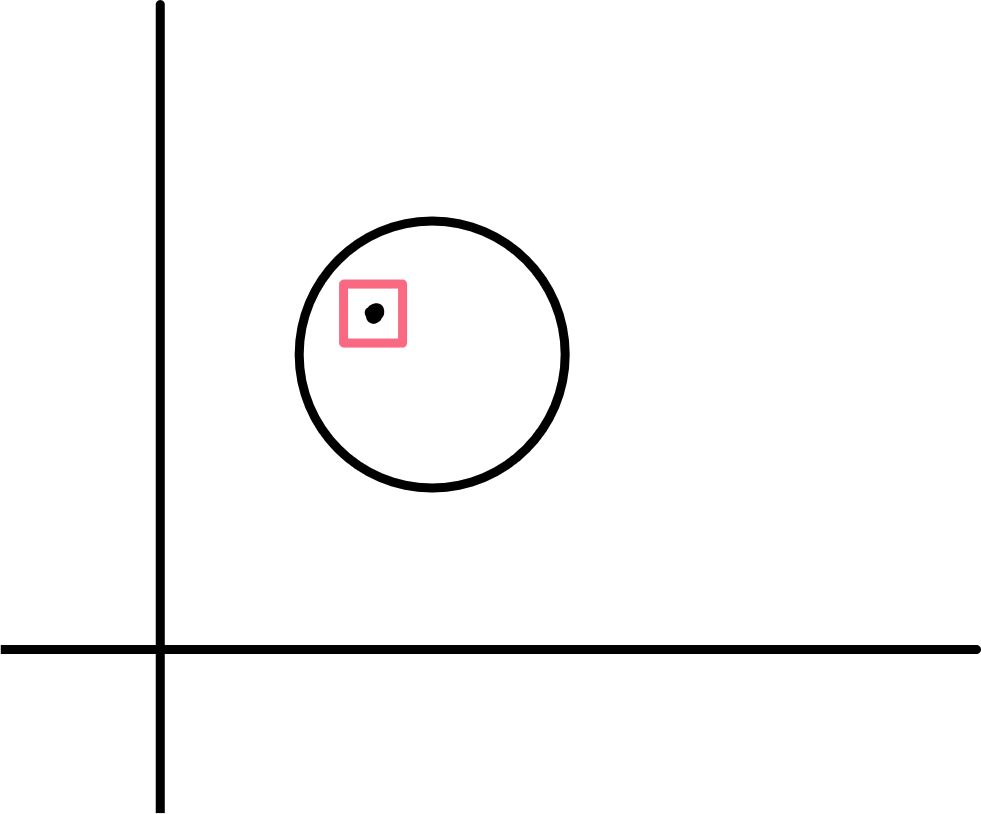
\includegraphics[height=5cm]{03-product}
\end{figure}

Thus, in general, we would want our product topology from $\tau,\sigma$ to be the collection of all union of sets in $\tau \times\sigma$.

\begin{definition}[$\pi$-system]
A \vocab{$\pi$-system} on a set $X$ is a non-empty subset $\pi\subset \mathcal{P}(X)$ such that $A,B\in \pi \implies A\cap B\in \pi$.
\end{definition}

\begin{proposition} \label{prp:37}
Let $\Pi$ be a $\pi$-system on a set $X$. Then
\begin{align*}
    \tau = \qty{\bigcup_{A\in \Sigma} A : \Sigma \subset \Pi} \cup \set{\emptyset, X}
\end{align*} is a topology on $X$.
\end{proposition}

\begin{proof}
Clearly, $\emptyset, X\in \tau$ and it's closed under arbitrary unions. \\
Now suppose $G,H \in \tau$.
If $G = \emptyset, X$ or $H = \emptyset, X$ then $G \cap H \in \tau$ trivially. \\
Otherwise $G = \bigcup_{A\in \Phi} A$, $H =\bigcup_{B \in \Theta} B$ for some $\Phi, \Theta \subset \Pi$.
Then $G \cap H = \bigcup_{A\in \Phi, B\in \Theta} (A \cap B) = \bigcup_{C \in \Sigma} C$, where $\Sigma = \Set{A \cap B}{A\in \Phi, B\in \Theta}\subset \Pi.$ Hence $G\cap H\in \tau$.
\end{proof}

\begin{definition}[Generated Topology]
We call this $\tau$ the topology \vocab{generated by} $\Pi$.
\end{definition}

\begin{proposition} \label{prp:38}
Let $(X,\tau), (Y,\sigma)$ be topological spaces. Then $\tau\times \sigma$ is a $\pi$-system on $X\times Y$.
\end{proposition}

\begin{proof}
$\emptyset = \emptyset \times \emptyset \in \tau\times \sigma$ so $\tau\times \sigma\neq \emptyset$. Now suppose $A,B\in\tau\times \sigma $. Then $A = G\times H$, $B=K\times L$ for some $G,K\in \tau$ and some $H,L,\in \sigma$. So $A\cap B = (G\cap K)\times (H\cap L) \in \tau\times \sigma$.
\end{proof}

\begin{definition}[Product Topology]
Let $(X,\tau), (Y,\sigma)$ be topological spaces. The \vocab{product topology} on $X\times Y$ is the topology generated by the $\pi$-system $\tau \times \sigma$.
\end{definition}
\begin{exercise*}
If $X=Y=\R$, $\tau=\sigma$ is the usual topology, show that the product topology on $\R^2$ is the Euclidean topology. (Sheet 3)
\end{exercise*}

\begin{theorem} \label{prp:39} ~\vspace*{-1.5\baselineskip}
\begin{enumerate}
    \item A product of Hausdorff spaces is Hausdorff.
    \item A product of compact spaces is compact.
\end{enumerate}
\end{theorem}

\begin{proof}
Let $(X,\tau), (Y,\sigma)$ be topological spaces and let $\rho$ be the product topology on $X\times Y$.
\begin{enumerate}
    \item Suppose $X,Y$ are Hausdorff. Let $(x,y), (z,w)\in X\times Y$ with $(x,y)\neq (z,w)$, wlog $x\neq z$. As $X$ is Hausdorff we can find $G,H\in \tau$ with $G\cap H = \emptyset$, $x\in G$, $z\in H$. Then $G\times Y, H\times Y\in \rho$ with $(G\times Y)\cap (H\times Y) = \emptyset$ and $(x,y)\in G\times Y$, $(z,w) \in H\times Y$. Thus $X\times Y$ is Hausdorff.
    \item Suppose $X\times Y$ compact. Let $\mathcal{C}\subset\rho$ be an open cover of $X\times Y$. Fix $x \in X$. For each $y\in Y$, there is some $G_y\in \mathcal{C}$ such that $(x,y)\in G_y$. Hence we can find $U_y\in \tau$ and $V_y\in \sigma$ such that $(x,y)\in U_y\times V_y\subset G_y$. In particular, we have $x\in U_y$ and $y\in V_y$. Thus $\Set{V_y}{y\in Y}\subset \sigma$ is an open cover of $Y$. So, as $Y$ is compact, it has a finite subcover $\set{V_{y_1},\dots, V_{y_n}}$, say.

    Let $W = \bigcap_{i=1}^n U_{y_i}$. Then $W$ is open in $X$ and $x\in W$. Moreover, $W\times Y \subset \bigcup_{i=1}^n (U_{y_i}\times V_{y_i}) \subset \bigcup_{i=1}^n G_{y_i}$. Now do this for each $x\in X$ to obtain $W_x = W, n_x = n$ and $G_{y_i}^{(x)} = G_{y_i}$ for ($1 \leq i  \leq n_x)$ as above. Then $\Set{W_x}{x\in X}\subset \tau$ is an open cover of $X$. So, as $X$ is compact, it has a finite subcover, $\set{W_{x_1},\dots , W_{x_m}}$, say.

    Now $X = \bigcup_{j=1}^m W_{x_j}$ and for each $j, W_{x_j}\times Y\subset \bigcup_{i=1}^{n_{x_j}} G_{y_i}^{(x_j)}$. Thus \[\Set{G_{y_i}^{(x_j)}}{1 \leq j \leq m, 1 \leq i \leq n_{x_j}}\] is an open cover of $X\times Y$ and hence a finite subcover of $\mathcal{C}$. Thus $X\times Y$ is compact.
\end{enumerate}
\end{proof}

\begin{remark}
    The second proof is a typical proof when working with products so it is useful to understand it and copy the idea.
\end{remark}

\subsection{Quotients}
Consider the surface of a torus (donut) in $\R^3$.
\begin{figure}[h]
    \centering
    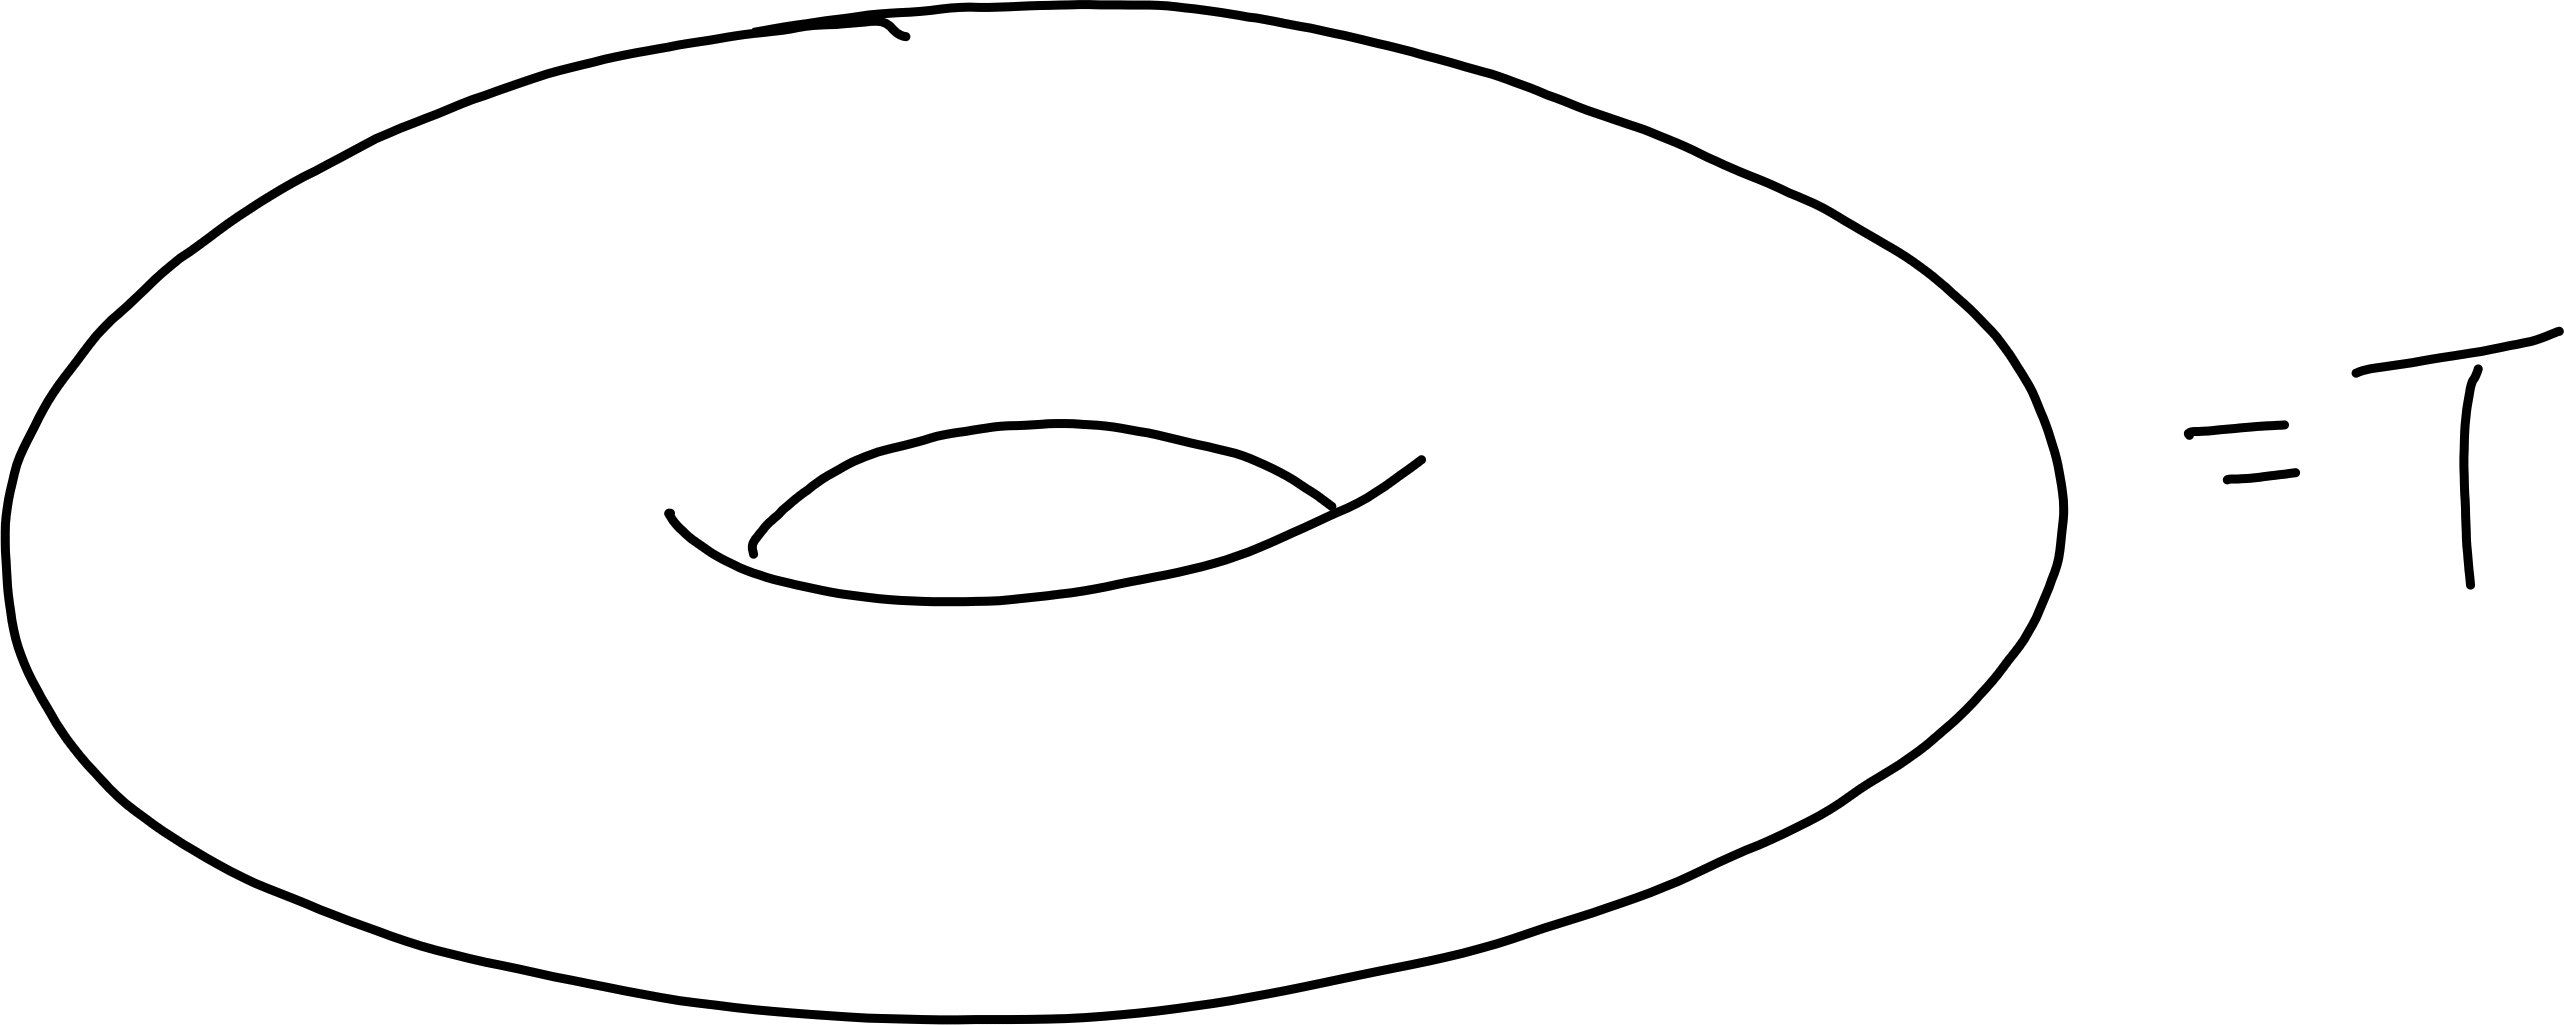
\includegraphics[height=5cm]{03-torus}
\end{figure}
We might be interested in for example, continuous functions $T\to T$. Analysis is likely to be unpleasant since the equation defining $T$ might be complicated. However, given that we care about continuity and convergence, if we replace $T$ by a space homeomorphic to $T$ then we're happy, particularly if the new space is analytically easier to work with.

For example take the closed unit square $[0,1]\times[0,1]$ with Euclidean subspace topology.
\begin{figure}[h]
    \centering
    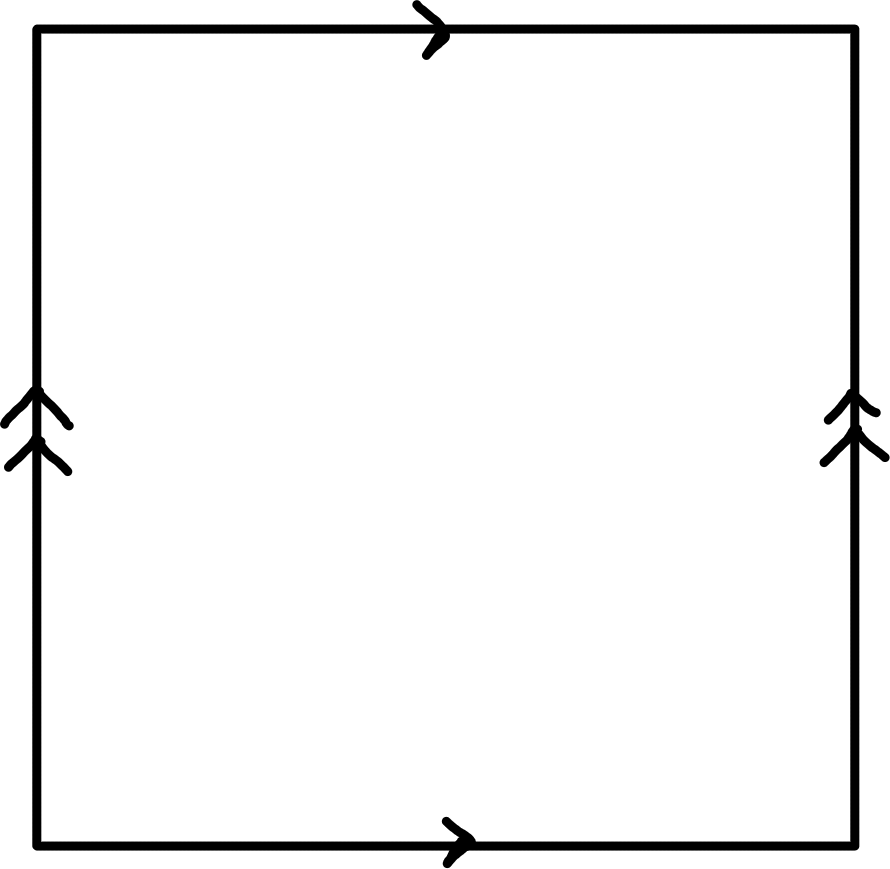
\includegraphics[height=5cm]{03-square}
\end{figure}
Glue $(x,0)$ to $(x,1)$ for each $x$, and glue $(0,y)$ to $(1,y)$ for each $y$; this seems to give us $T$. More specifically, we defined an equivalence relation on $[0,1]\times[0,1]$, say by $\sim$, with equivalence classes:
\begin{align*}
    \set{(x,y)} & \quad 0<x,y<1\\
    \set{(x,0),(x,1)} & \quad 0<x<1\\
    \set{(0,y),(1,y)} & \quad 0<y<1\\
    \set{(0,0), (0,1), (1,0), (1,1)}.
\end{align*}
Essentially we could define $T = [0,1]^2 / {\sim}$, the set of equivalence classes.
This definition seems annoying - a better one could perhaps be defining an equivalence relation $\sim$ on $\R^2$, where every unit square is ``mapped'' to the $[0,1]$ square, i.e. $(x,y)\sim(z,w) \Leftrightarrow x-z\in \mathbb{Z}$ and $y-w\in \mathbb{Z}$.
\begin{figure}[h]
    \centering
    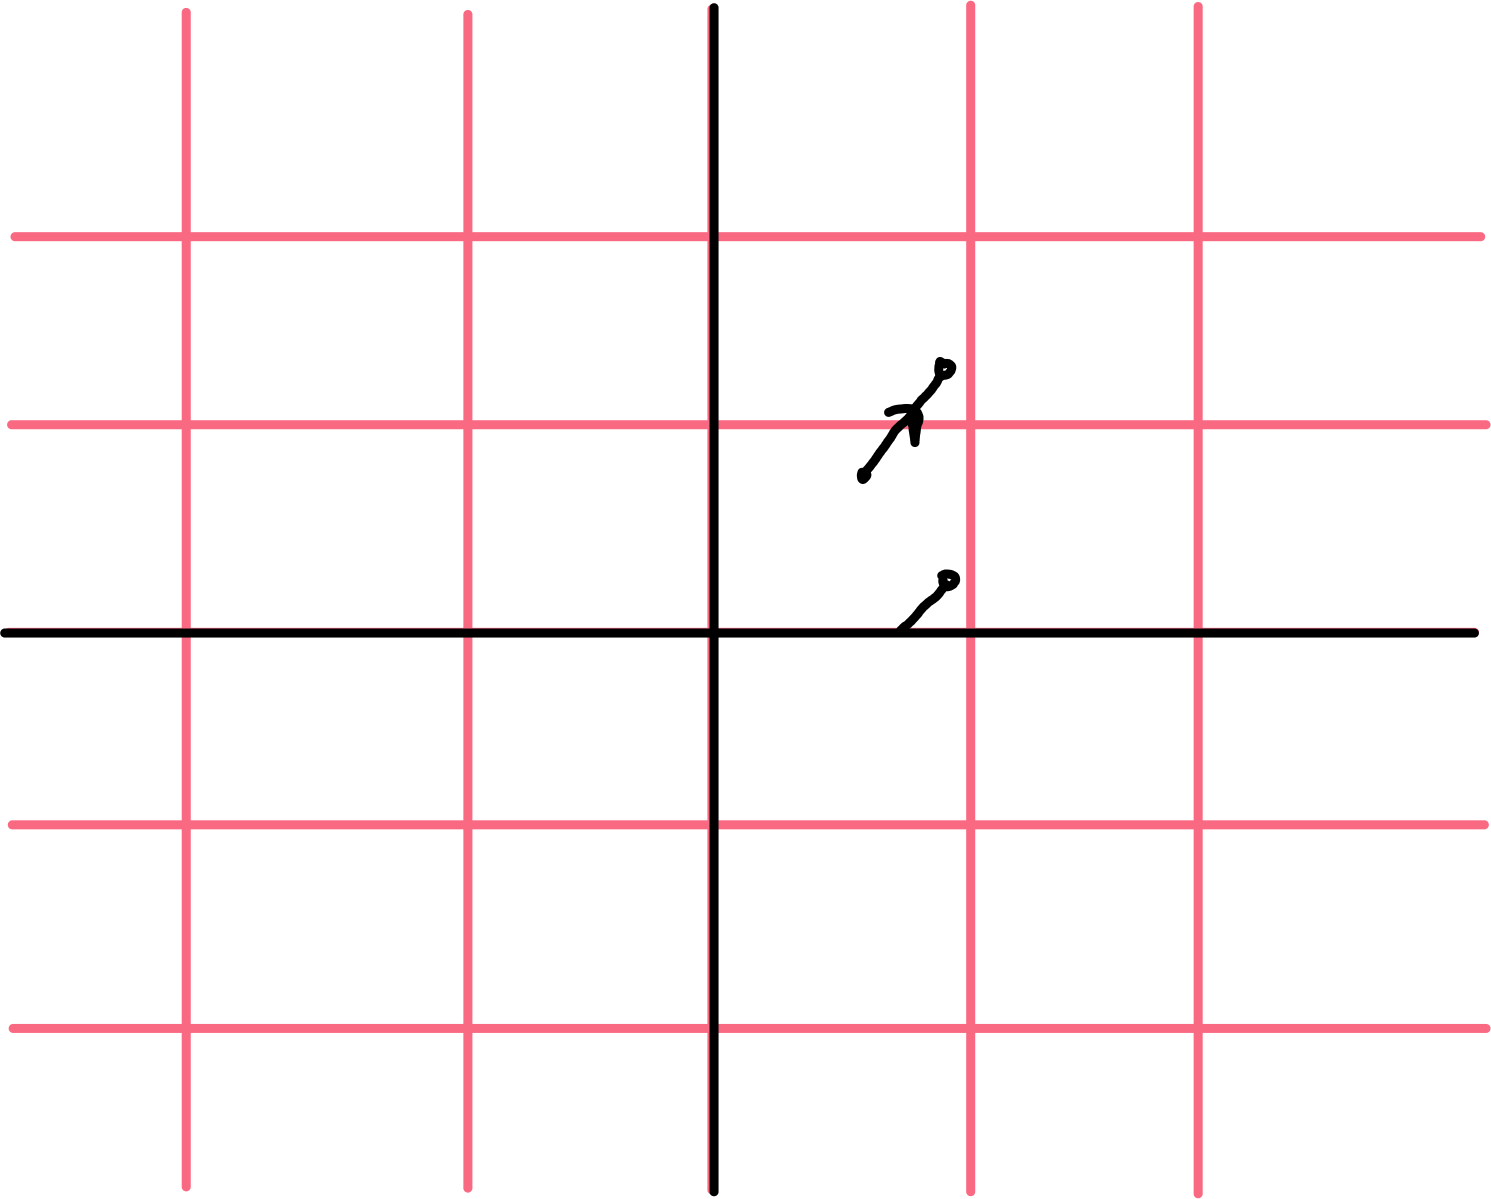
\includegraphics[height=5cm]{03-squareongrid}
    \caption{The squares `wrap' over.}
\end{figure}
Again, hopefully we can define $T = R^2/ {\sim}$. \\
\underline{But} what is the topology?
\begin{definition}[Quotient Topology]
    Let $(X,\tau)$ be a topological space and let $\sim$ be an equivalence relation on $X$. Let $q: X\to X/ {\sim}$ be the quotient map, i.e. $\forall x \in X,\ q(x) = [x]_\sim$ (equivalence class of $x$).
    The \vocab{quotient topology} on $X/ {\sim}$ is
    \begin{align*}
        \rho = \Set{G\subset X/ {\sim}}{q\inv(G)\in \tau}
    \end{align*}
\end{definition}

\begin{remark}
    \begin{enumerate}
        \item $\rho$ is indeed a topology using $q\inv(\bigcup G) = \bigcup q\inv(G)$ and $q\inv (G\cap H) = q\inv(G)\cap q\inv (H)$.

        \item $\rho$ is the largest topology on $X/ {\sim}$ making the quotient map $q$ continuous.
    \end{enumerate}
\end{remark}

\begin{example}
    Take $\R$ with the usual topology and $X\sim Y$ iff $x-y\in \Z$.
    Then $\R/ {\sim}$ `is' $S^1$, the unit circle (a subspace of $\R^2$ with the Euclidean topology), where `is' means `is homeomorphic to'.
    We will prove this later.
\end{example}

\begin{example}
    Suppose as above, but now $x\sim y$ iff $x-y\in \Q$. What is the quotient topology on $\R/ {\sim}?$
    Suppose $G\subset \R/ {\sim}$ is open and $G\neq \emptyset$.
    Then $q\inv (G)\subset\R$ is open and non-empty so contains some interval $(a,b)\subset q\inv (G)$ with $a\neq b$.
    Now take any $x\in \R$, then $\exists y\in (a,b)$ with $x-y\in \mathbb{Q}$ i.e. $x\sim y$.
    Then $q(x) = [x]_\sim = [y]_\sim \in G$. Hence $G = \R/ {\sim}$.

    So quotient topology on $\R/ {\sim}$ is the indiscrete topology.
\end{example}

\begin{example}
    Quotients of metrizable spaces need not be metrizable, and the same holds if `metrizable' is replaced with `Hausdorff'.
\end{example}

\subsubsection{Basics on equivalence relations and quotients}

Suppose $X$ is a set and $\sim$ is an equivalence relation on $X$. We have $X/ {\sim} = \Set{[x]_\sim}{x\in X}$ and have quotient map $q:X \to X/ {\sim},$ $x \mapsto [x]_\sim$. Clearly $q$ is surjective.

Suppose now $Y$ is also a set and $f:X\to Y$. Assume $f$ \vocab{respects} $\sim$, i.e. $x\sim y \implies f(x) = f(y)$.
% https://q.uiver.app/?q=WzAsMyxbMCwwLCJYIl0sWzEsMSwiWC8ge1xcc2ltfSJdLFsyLDAsIlkiXSxbMCwxLCJxIiwyXSxbMSwyLCJcXGJhcntmfSIsMix7InN0eWxlIjp7ImJvZHkiOnsibmFtZSI6ImRhc2hlZCJ9fX1dLFswLDIsImYiXV0=
\[\begin{tikzcd}
	X && Y \\
	& {X/ {\sim}}
	\arrow["q"', from=1-1, to=2-2]
	\arrow["{\bar{f}}"', dashed, from=2-2, to=1-3]
	\arrow["f", from=1-1, to=1-3]
\end{tikzcd}\]
Then there is a unique function $\bar{f}: X/ {\sim} \to Y$ such that $f = \bar{f}\circ q$.
Indeed, we must have $\forall \; x \in X$ $\bar{f}([x]_\sim) = \bar{f}(q(x)) = f(x)$.
As $f$ respects $\sim$, this is well defined: $[x]_\sim = [y]_\sim \implies x \sim y \implies f(x) = f(y)$.

\begin{example}
Suppose $G,H$ are groups and $\theta: G\to H$ is a homomorphism. Let $K = \ker\theta$, and define $\sim$ on $G$ by $g\sim h\Leftrightarrow g\inv h\in K$. Then $G/K = G/ {\sim}$ and consider $\bar{\theta}: G/K\to H$.
% https://q.uiver.app/?q=WzAsNCxbMCwwLCJHIl0sWzEsMSwiRyAvIEsiXSxbMiwwLCJIIl0sWzEsMF0sWzAsMSwicSIsMl0sWzEsMiwiXFxiYXJ7XFx0aGV0YX0iLDIseyJzdHlsZSI6eyJib2R5Ijp7Im5hbWUiOiJkYXNoZWQifX19XSxbMCwyLCJcXHRoZXRhIl1d
\[\begin{tikzcd}
	G & {} & H \\
	& {G / K}
	\arrow["q"', from=1-1, to=2-2]
	\arrow["{\bar{\theta}}"', dashed, from=2-2, to=1-3]
	\arrow["\theta", from=1-1, to=1-3]
\end{tikzcd}\]
We can check that $\bar{\theta}$ is a homomorphism and injective thus isomorphism onto $\theta(G)$. This is the first isomorphism theorem.
\end{example}

\begin{proposition} \label{prp:40}
    Let $(X,\tau)$ be a topological space and $\sim$ be an equivalence relation on $X$. Let $\rho$ be the quotient topology on $X/ {\sim}$. Suppose $f: X\to Y$ is a continuous function respecting $\sim$, where $(Y,\sigma)$ is a topological space. Then there is a unique continuous function $\bar{f}:X/ {\sim}\to Y$ such that $f = \bar{f}\circ q$, where $q: X\to X/ {\sim}$ is a quotient map.
\end{proposition}

\begin{proof}
Define $\bar{f}: X/ {\sim}\to Y$ by $\bar{f}([x]_\sim) = f(x)$. \\
This is well-defined, $[x]_\sim = [y]_\sim \implies x\sim Y \implies f(x) = f(y)$.
Clearly $\bar{f}\circ q=f$.
Let $G\in \sigma$. Then $q\inv(\bar{f}\inv(G)) = (\bar{f}\circ q)\inv (G) = f\inv (G)\in \tau$ as $f$ is continuous.
So by definition of quotient topology, $\bar{f}\inv(G)\in \rho$.
Hence $\bar{f}$ is continuous.

Finally, if $f = h \circ q$ for some $h:X/ {\sim}\to Y$ then $\forall x\in X$, $h([x]_\sim) = h(q(x)) = f(x) =\bar{f}([x]_\sim)$. So $h = \bar{f}$.
\end{proof}

\begin{remark}
This is what makes quotients useful.
E.g. recall torus $T = \R^2/ {\sim}$ for an appropriate relation $\sim$.
Hopefully $T$ is homeomorphic to a genuine torus as a surface in $\R^3$, e.g. $T$ is nasty while $R^2$ is nice.
Hence we want to work `upstairs' in $R^2$ rather than `downstairs' in $T$.
For examples, if you want to think about a continuous function on $T$, we can instead think about an appropriate continuous function on $\R^2$ respecting $\sim$.
\end{remark}

\begin{example}
Recall we had $\R$ with the usual topology, $x\sim y$ iff $x-y\in \Z$ and $S^1= $ $ \Set{x\in \R^2}{||x||=1}$ with subspace topology inherited from Euclidean topology on $\R^2$. \\
We claimed $\R/ {\sim}$ is homeomorphic to $S^1$. Define $f:\R \to S^1$ by $f(x) = (\sin 2\pi x, \cos 2\pi x)$.
Clearly $f$ is a continuous surjection and it respects $\sim$.
By \cref{prp:40} there is a unique continuous $\bar{f}: \R/ {\sim} \to S^1$ with $\bar{f}\circ q = f$.

Clearly $\bar{f}$ is a continuous bijection (for injectivity, note each $x\in S^1$ is $f(a)$ for unique $a\in[0,1)$ and each $b\in \R$ has $b\sim a$ for a unique $a\in[0,1)$).

Now $\R/ {\sim} = q([0,1])$ is a continuous image of a compact set and so is compact. And $S^1$ is Hausdorff as its a metric space.
We also know that any continuous bijection from a compact space to a Hausdorff space is a homeomorphism.

Thus we are done, as $\bar{f}$ is a homeomorphism from $\R/ {\sim}$ to $S^1$.
\end{example}

\subsection{Connectedness}

Recall the \emph{Intermediate Value Theorem} (IVT): if $f:[a,b]\to \R$ is continuous and wlog $f(a)<f(b)$ then $[f(a),f(b)]\subset f([a,b])$. \\
Moreover, if $c,d \in f([a,b])$ with $c<d$ then $[c,d]\subset f([a,b])$.

However, this doesn't work more generally, e.g. if we replace $[a,b]$ by $[-1,0)\cup (0,1] = X$. Define $f:X\to \R$ by \begin{align*}
    \begin{cases}
        1 & x<0\\
        0 & x>0.
    \end{cases}
\end{align*}
Then $f$ is continuous on $X$, $0\in f(X)$, $1\in f(X)$, but e.g. $1/2 \not\in f(X)$ so $[0,1] \not\subset f(X)$. Indeed, this is because $[-1,0)\cup (0,1]$ is `disconnected'.

\begin{definition}[Connectedness]
A topological space $X$ is \vocab{disconnected} if there exist disjoint, non-empty open sets $U,V$ with $X = U\cup V$.
We say $X$ is \vocab{connected} if $X$ is not disconnected.
\end{definition}

\begin{remark}
    \begin{enumerate}
        \item Recall that $U\subset X$ is closed iff its complement, $X \setminus U$ is open. \\
        If $X$ is disconnected then $X = U \cup V$ so $U = X \setminus V$ and $V = X \setminus U$, so $U, V$ closed.
        Thus, $X$ is disconnected iff there exist disjoint, non-empty closed sets $U,V$ with $X = U\cup V$.

        Further, if there exist an open and closed set of $X$, say $A$, then $A \cup (X \setminus A) = X$.
        So $X$ is connected iff the only subsets of $X$ that are both open and closed are $\emptyset, X$.

        $X$ is connected iff whenever $U,V\subset X$ are open and disjoint with $X=U\cup V$ then $U=\emptyset$ or $V=\emptyset$. Again, we could replace `open' by `closed'.

        If $X$ is disconnected, we say the sets $U,V$ in the definition \vocab{disconnect} $X$.

        \item Connectedness is a topological property.
        \item if $S\subset X$, where $X$ is a topological space, what does our definition of connectedness say when applied to $S$? Of course, as usual $S$ has the subspace topology from $X$ so is a topological space in its own right.

        $S$ is disconnected $\iff$ there exist open sets $U,V\subset X$ such that $(S \cap U) \cap (S \cap V) = S\cap U\cap V = \emptyset$, $S \cap U, S \cap V \neq \emptyset$ and $(S \cap U) \cup (S \cap V) = S$ i.e. $S\subset U\cup V$. Again, we say $U,V$ disconnect $S$.

        \begin{warning}
            It is not necessary to have $U\cap V =\emptyset$, e.g. in $\N$ with cofinite topology, the set $\set{1,2}$ is disconnected in $\N$ by the open sets $\N\setminus \set{1}, \N\setminus \set{2}$. We have $(\N\setminus \set{1}) \cap (\N\setminus \set{2})\cap \set{1,2} = \emptyset$ but $(\N\setminus \set{1})\cap (\N\setminus \set{2}) \neq \emptyset$. Indeed, if $U,V\subset \N$ are open and non-empty then $U\cap V\neq\emptyset$ (if $U, V$ open in cofinite topology then they have finite complement so their intersection has finite complement.).
        \end{warning}

        Thus $S$ is connected iff whenever $U,V\subset X$ are open, $S\cap U\cap V=\emptyset$ and $S \subset U \cup V$ then either $S\cap U=\emptyset$ or $S\cap V=\emptyset.$

        Finally, as in remark 1, could replace `open' with `closed' in these reformulations of the definition.
    \end{enumerate}
\end{remark}

\begin{question}
    Which subsets of $\R$ are connected?
\end{question}

\begin{definition}[Interval]
    A subset $I\subset \R$ is an \vocab{interval} if whenever $a<b<c$ with $a, c \in I$ then $b \in I$.
\end{definition}

\begin{proposition} \label{prp:41}
    Let $I\subset \R$ with the usual topology. Then $I$ is connected iff $I$ is an interval.
\end{proposition}

\begin{proof}
    ($\implies$): Suppose $I$ is not an interval. Then we can find $a<b<c$ with $a,c\in I$ but $b\not\in I$. Then $(-\infty,b)$ and $(b,\infty)$ disconnect $I$ in $\R$.

    ($\Longleftarrow$): Suppose $I$ is an interval. Work in the subspace topology on $I$. Let $S\subset I$ be open, closed and non-empty. Let $a\in S$. \\
    Suppose we have $b\in I\setminus S$. Wlog $b>a$. Let $c=\sup([a,b]\cap S)$. Then we can find a sequence $(x_n)$ in $S$ with $x_n\to c\in I$. But $S$ is closed in $I$ so $c\in S$. In particular, $c\neq b$. so $c<b$.

    But also $S$ is open in $I$ so $\exists \delta>0$ such that $(c-\delta, c+\delta)\subset S$, wlog $\delta < b-c$. Then $c +\frac{\delta}{2}\in S\cap [a,b]$ \Lightning.
    Thus in fact, $S=I$ and hence $I$ is connected.
\end{proof}

\begin{theorem}[Equivalent definition of connectedness] \label{thm:42}
    Let $X$ be a topological space. Then $X$ is connected iff every continuous $f: X\to \Z$ (with the usual topology) is constant.
\end{theorem}

\begin{proof}
    ($\implies$): Suppose $X$ is connected and $f:X\to \Z$ continuous. For any $n\in \Z$, $\set{n}\subset \Z$ is open and closed so $f\inv(\set{n})\subset X$ is open and closed, so $f\inv(\set{n})= \emptyset$ or $f\inv(\set{n}) = X$\footnote{Connectedness implies only open and closed subsets of $X$ are $\emptyset, X$.}. Thus $f$ is constant.

    ($\Longleftarrow$): Suppose $U,V$ disconnect $X$. Define $f:X \to \mathbb{Z}$ by $f(x) = \begin{cases}
        0 & x \in U \\
        1 & x \in V
    \end{cases}$.
    Then for any $A\subset \Z$, $f\inv(A) = \emptyset,X,U$ or $V$\footnote{We get $\emptyset$ if $0, 1 \notin A$, $X$ if $\{0, 1\} \subset A$, \dots} and so $f\inv(A)$ is open. So $f$ is continuous and non-constant.
    \end{proof}

    \begin{remark}
    1. \Cref{thm:42} together with the IVT can provide an alternative proof of \cref{prp:41}.

    2. \Cref{thm:42} remains true with same proof if $\Z$ is replaced by any discrete topological space $Y$ with $|Y| \geq 2$ (need two points to construct $f(x)$ in ($\Longleftarrow$)).
\end{remark}

\begin{proposition} \label{prp:43}
    A continuous image of a connected space is connected.
\end{proposition}

\begin{proof}
    Let $X$ be a connected topological space, let $Y$ be a topological space and let $f:X\to Y$ be continuous. Suppose $U,V\subset Y$ are open with $f(X)\subset U\cup V$ and $U\cap V\cap f(X) = \emptyset$.

    As $f$ is continuous, $f\inv(U),f\inv(V)\subset X$ are open. Also $X = f\inv(U)\cup f\inv(V)$ and $f\inv(U) \cap f\inv(V)=\emptyset$. As $X$ is connected, wlog $f\inv(U)= \emptyset$. Then $U \cap f(X)=\emptyset$. So $f(X)$ is connected.
\end{proof}

\begin{proposition} \label{prp:44}
    A product of connected spaces is connected.
\end{proposition}

\begin{proof}
    Let $(X,\tau)$ and $(Y,\sigma)$ be connected topological spaces, and let $\rho$ be the product topology on $X\times Y$.

    Suppose $U,V\in\rho$ with $U\cap V=\emptyset$ and $U\cup V = X\times Y$. We want to show $U=\emptyset$, $V=X\times Y$ or $U=X\times Y$, $V=\emptyset$.

    Fix $x\in X$. Then $\set{x}\times Y$ is homeomorphic to $Y$ (Sheet 3). In particular, $\set{x}\times Y$ is connected. Then $\set{x}\times Y\subset U$ or $\set{x}\times Y \subset V$ as otherwise $U,V$ would disconnect $\set{x}\times Y$ in $X\times Y$.

    Let $A = \Set{x\in X}{\set{x}\times Y\subset U}$ and $B = \Set{x\in X}{\set{x}\times Y \subset V}$. Clearly $A\cap B = \emptyset$ (as $U\cap V = \emptyset)$ and we've proved that $X = A\cup B$. Now we want to show that $A,B$ are open to use connectedness in $X$.

    Suppose $x\in A$. Then $\set{x}\times Y\subset U$. Then (assuming $Y\neq \emptyset$, which we do wlog) pick any $y\in Y$. Then $(x,y)\in U$. $U$ is open so can find $T\in \tau$, $S\in \sigma$ such that $(x,y)\in T\times S \subset U$.
    In particular, for all $w \in T$ then $(w,y) \in U$ and so $\set{w}\times Y\subset U$\footnote{If $\set{w} \times \set{y} \in U$ and $\set{w} \times \set{a} \in V$ for some $a \in Y$ this contradicts $\set{x} \times Y \subset U$ or $\set{x} \times Y \subset V$.}, i.e. $w \in A$. We now have $T\in \tau$ with $x\in T\subset A$ so $A$ is a neighbourhood of $x$ in $X$. Hence $A$ is open.

    Similarly $B$ is open. Since $X$ is connected, so $A=\emptyset$ giving $U=\emptyset$ or $B=\emptyset$ giving $V=\emptyset$. Hence $X\times Y$ is connected.
\end{proof}

\begin{example}[What can we do with spaces that aren't connected?]
    Recall $[-1,0)\cup (0,1]$ is not connected. But it \underline{is} a disjoint union of connected sets. Moreover, any proper superset of $[-1,0)$ or $(0,1]$ in $[-1,0) \cup (0,1]$ is disconnected.

    We see here that the space is not connected, but we can take two maximal subsets of the space that are connected that gives us the entire space.
\end{example}

\begin{definition}[Connected Component]
    Let $X$ be a topological space. A \vocab{connected component} of $X$ is a maximal connected subset $A$ of $X$: that is to say, $A$ is connected but if $A\subset B\subset X$ with $B$ connected then $A=B$.
\end{definition}

\begin{theorem} \label{thm:45}
    The connected components of a topological space $X$ form a partition of $X$.
\end{theorem}

\begin{proof}
    Define $\sim$ on $X$ by $x\sim y$ iff $\exists A\subset X$ connected with $x,y \in A$.
    Clearly $\sim$ is reflexive ($\set{x}$ connected) and symmetric.
    Let's check that it is transitive.

    Suppose $x,y,z\in X$ with $x\sim y$ and $y\sim z$.
    Then $\exists A,B\subset X$ connected with $x,y\in A$ and $y,z\in B$. Now $x,z\in A\cup B$. Suppose $U,V$ disconnect $A\cup B$ in $X$.
    Wlog $y\in U$. Pick $w\in V\cap(A\cup B)$.
    Wlog $w\in A$. But also $y\in A$ so $U,V$ disconnect $A$ \Lightning.
    So $A\cup B$ is connected, so $x\sim z$, thus $\sim$ is indeed an equivalence relation.

    Now suppose $S$ is an equivalence class of $\sim$.
    We want to show that $S$ is connected.
    Suppose $U,V$ disconnect $S$. Then we can find $x\in U\cap S$, $y\in V\cap S$ and $U\cap V\cap S = \emptyset$.
    Then $x\sim y$ so there is a connected $A\subset X$ with $x,y\in A$.
    For all $z\in A$, $x,z\in A$ are connected so $x\sim z$ so $z\in S$.
    So $A\subset S$ and so $U\cap V\cap A = \emptyset$ which gives $U,V$ disconnects $A$ \Lightning.
    Hence $S$ is connected.

    Now let's show $S$ is a connected component. Suppose $S\subset T\subset X$ with $T$ connected.
    Let $x\in S$. Then for all $y\in T$, $x,y\in T$ with $T$ connected so $x\sim y$.
    Thus $T\subset S$, so $S=T$ and $S$ is a connected component.

    Finally let $R$ be a connected component and let $x,y\in R$. Then, as $R$ is connected, $x \sim y$.
    So $R$ is contained in some equivalence class $Q$ of $\sim$.
    But $R\subset Q$ with $Q$ connected so $R=Q$. Hence equivalence classes of $\sim$ are precisely the connected components.
\end{proof}

Another concept of connectedness:
\begin{remark}
    This is what tells us connected components exist.
\end{remark}

\begin{definition}[Paths]
    A \vocab{path} from $x$ to $y$ in a topological space $X$ is a continuous function $\phi:[0,1]\to X$ with $\phi(0) = x$, $\phi(1) = y$.
\end{definition}

\begin{definition}[Path-Connected]
    $X$ is \vocab{path-connected} if for all $x,y\in X$ there is a path from $x$ to $y$.
\end{definition}

\begin{proposition} \label{prp:46}
    A path-connected space $X$ is connected.
\end{proposition}

\begin{proof}
    Suppose $U,V$ disconnect $X$. Pick $a\in U, b\in V$. Let $\phi$ be a path in $X$ from $a$ to $b$. Then $U,V$ disconnect $\phi([0,1])$ \Lightning.
\end{proof}

\begin{warning}
    The converse is not true!
\end{warning}

\begin{example}
Consider
{\par
\centering
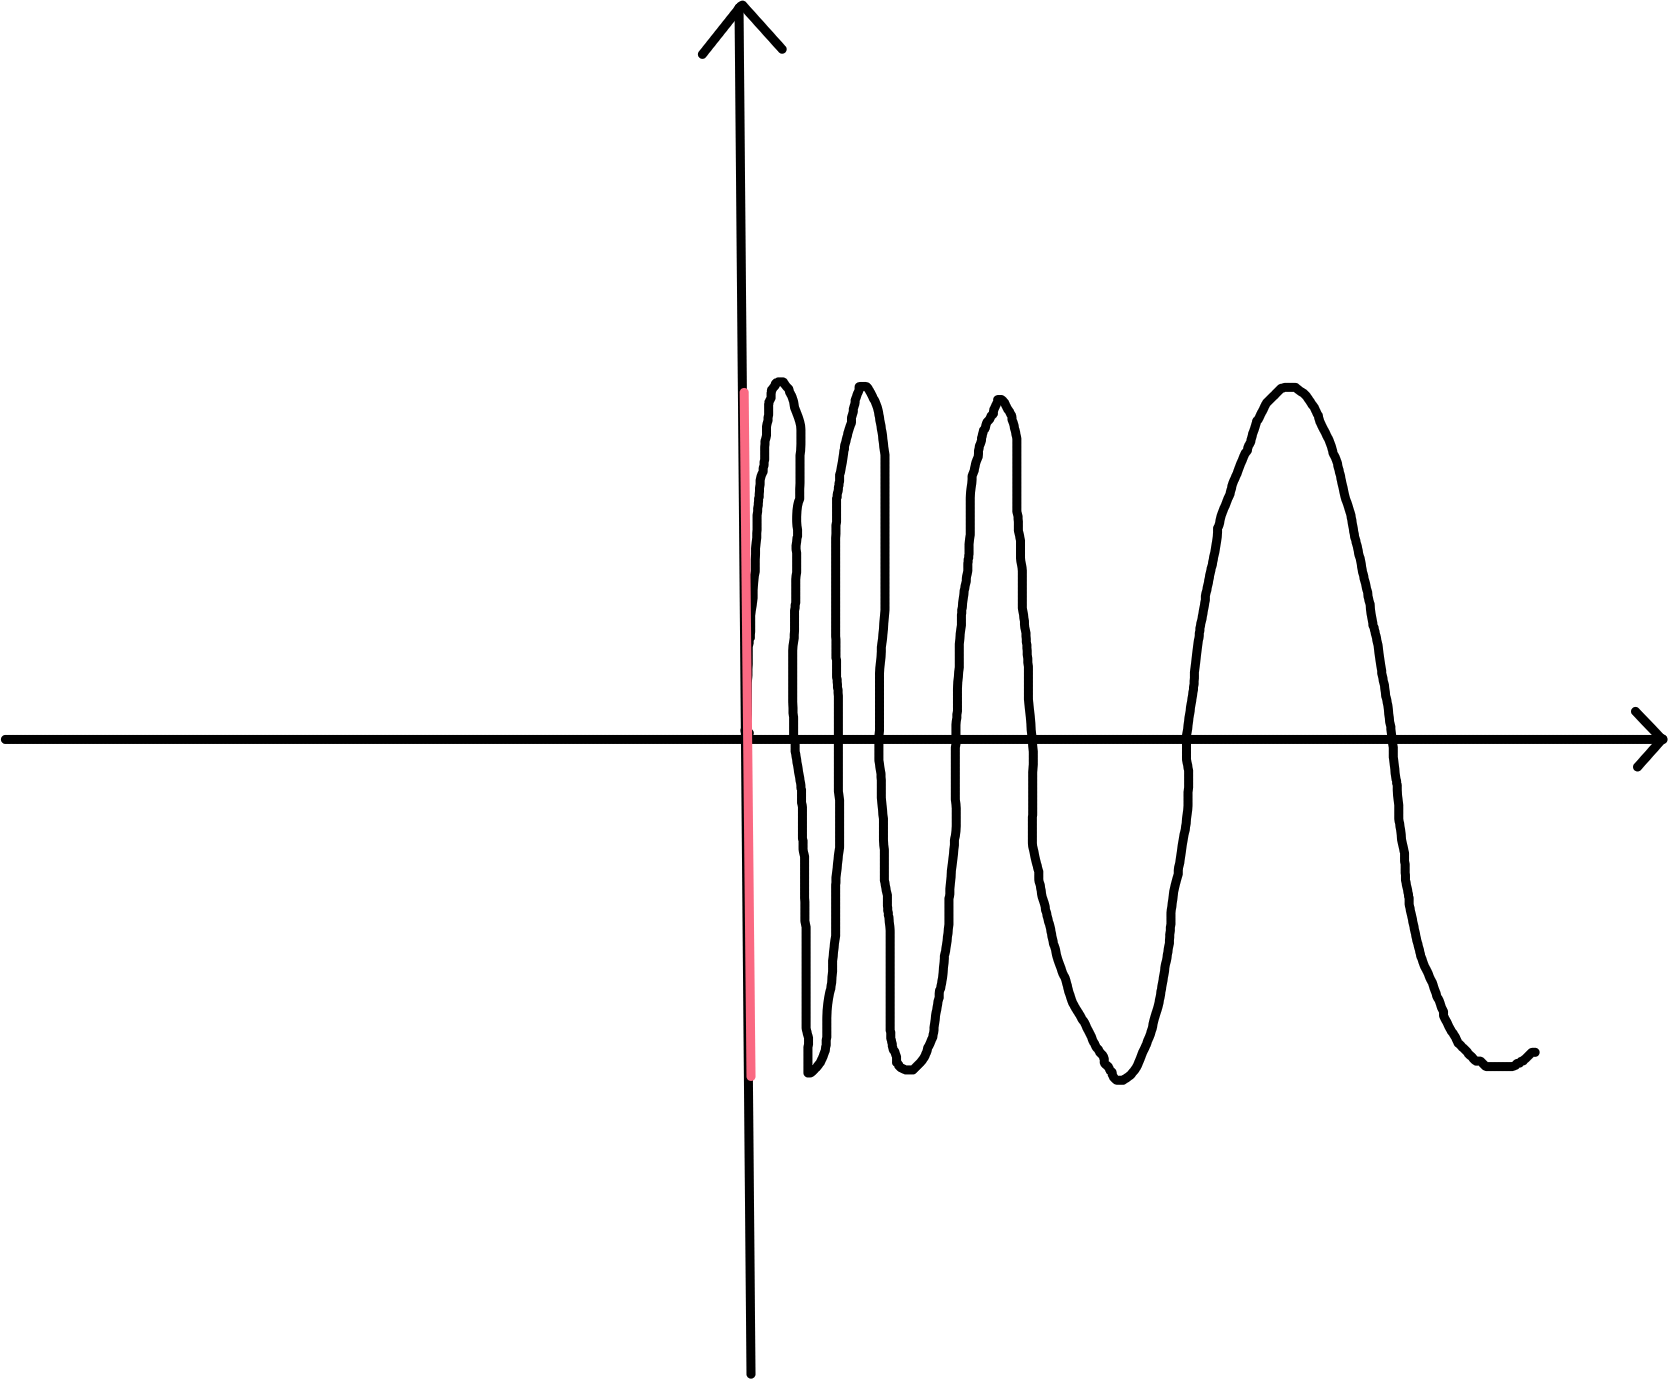
\includegraphics[height=5cm]{03-connected}
\par}
\begin{align*}
    A &= \Set{(0,y)}{-1\leq y \leq 1} \\
    B &= \left\{ \qty(x,\sin \frac{1}{x}) : 0< x\leq 1 \right\}
\end{align*}
and $X = A\cup B \subset \R^2$. Let's show that $X$ is connected but not path-connected.
\end{example}

\begin{claim}
    $X$ connected.
\end{claim}

\begin{proof}
    Clearly $A,B$ themselves are path-connected so connected.
    Suppose $U,V$ disconnect $X$ in $\R^2$.
    Then wlog $A\subset U$, $B\subset V$.
    So $(0,0)\in A\subset U$. $U$ is open so there exists $\delta>0$ such that $B_\delta((0,0))\subset U$.
    Pick $n$ such that $\frac{1}{2n\pi}<\delta$. Then $(\frac{1}{2n\pi},0)\in U\cap B$ \Lightning.
\end{proof}

\begin{claim}
    $X$ not path-connected.
\end{claim}

\begin{proof}
    Suppose $\phi$ is a path from $(0,0)$ to $(1,\sin 1)$ in $X$.
    Let $\sigma = \sup\Set{t\in [0,1]}{\phi_1(t) = 0}$.
    Let $y = \phi_2(\sigma)$.
    Then, as $\phi$ is continuous, $\phi(\sigma) = (0,y)$.

    Choose $\delta > 0$ such that $|\sigma - t| <\delta \implies \norm{\phi(\sigma) - \phi(t)} < 1$.
    Wlog $\delta < 1-\sigma$. By definition of $\sigma$, $\phi_1(\sigma + \frac{\delta}{2}) = x > 0$.
    Choose $w\in (0,x)$ such that $\abs{\sin \frac{1}{w} - y} \geq 1$.
    Then by IVT, there is some $t\in \qty(\sigma, \sigma +\frac{\delta}{2})$ such that $\phi_1(t) = w$. Then $\abs{\sigma - t} < \delta$ but $\norm{\phi(\sigma) - \phi(t)} \geq \abs{\phi_2(\sigma) - \phi_2(t)} = \abs{\sin\frac{1}{w} - y} \geq 1$ \Lightning.
\end{proof}

\begin{proposition} \label{prp:47}
    An open, connected subset of Euclidean space is path-connected.
\end{proposition}

\begin{proof}
    Let $X\subset \R^n$ be open and connected.
    If $X = \emptyset$ we are done.
    So assume $X \neq \emptyset$.

    Fix $a \in X$ and let \[ U = \Set{x\in X}{\exists \textup{ path in } X \textup{ from } a \textup{ to } x}. \]
    Note that $U\neq \emptyset$ as $a\in U$, since  there is a constant path from $a$ to $a$.

    \begin{claim}
        $U$ open in $X$.
    \end{claim}
    \begin{proof}
    Suppose $b\in U$.
    Since $X$ is open we can pick $\delta > 0$ such that $B_\delta(b) \subset X$.
    Let $\phi$ be a path from $a$ to $b$ in $X$ and let $x \in B_\delta(b)$.
    Then $\theta$ is a path in $X$ from $a$ to $x$ where
    \begin{align*}
        \theta(t) = \begin{cases}
        \phi(2t) & 0\leq t \leq \frac{1}{2}\\
        b + 2(t-\frac{1}{2})(x-b) & \frac{1}{2}\leq t \leq 1
        \end{cases}.
    \end{align*}
\end{proof}

\begin{claim}
    $U$ closed in $X$, i.e. $X\setminus U$ is open in $X$.
\end{claim}

\begin{proof}
    Let $b \in X \setminus U$.
    Choose $\delta> 0$ such that $B_\delta(b) \subset X.$ Suppose $x\in B_\delta (b)\cap U$.
    Let $\phi$ be a path in $X$ from $a$ to $x$. Then
    \begin{align*}
        t \mapsto \begin{cases}
        \phi(2t) & 0\leq t \leq \frac{1}{2}\\
        b + 2(t-\frac{1}{2})(b-x) & \frac{1}{2}\leq t \leq 1
        \end{cases}
    \end{align*}
    is a path from $a$ to b in $X$ \Lightning.
    Thus $B_\delta (b) \subset X\setminus U$.
    \end{proof}
    Hence, as $X$ is connected, $U=X$.
    But the point $a$ was arbitrary.
    Thus $X$ is path-connected.
\end{proof}

\begin{remark}
    Recall that we don't always specify the topology when defining a topological space; we should always assume it's the standard one. In particular, $\mathbb{R}$ comes with the usual topology, and $\mathbb{R}^n$ comes with the Euclidean topology. $X\subset \mathbb{R},\mathbb{R}^n$ comes with the subspace topology from their standard topologies.

    Products/Quotients come with the product/quotient topology respectively.
\end{remark}